\documentclass{tufte-handout}


\usepackage{style}
\newcommand*{\Ph}{\hphantom{)}}%

\newenvironment{amatrix}[1]{%
  \left(\begin{array}{@{}*{#1}{c}|c@{}}
}{%
  \end{array}\right)
}

\newenvironment{longdiv}[1]{%
  \(\begin{array}{r@{}*{#1}{c} r r}
}{%
  \end{array}\)
}

% Custom polynomial long division layout
\newcommand{\myPolyDiv}[2]{%
  \setlength{\arraycolsep}{2pt}%
  \renewcommand{\arraystretch}{1.1}%
  \begin{array}{rrrrrrr}
      & & & & & 5x & +4
  \end{array}\\[-2pt]
  \begin{array}{rrr|rrrr}
    \cmidrule{4-7}
    #2 & #1 \\
  \end{array}\\[-2pt]
  \begin{array}{rrrrrrr}
      & & & -5x^{3} & +15x^{2} & +90x & \\
    \cmidrule{4-6}
      & & & & 4x^{2} & -9x & -72 \\
      & & & & -4x^{2} & +12x & +72 \\
    \cmidrule{5-7}
      & & & & & 3x & 0 \\
  \end{array}}

% Custom polynomial long division layout
\newcommand{\myPolyDiv2}[2]{%
  \setlength{\arraycolsep}{2pt}%
  \renewcommand{\arraystretch}{1.1}%
  \begin{array}{r@{}r@{}r@{}r@{}r@{}r@{}r@{}}
      & & & & & 5x & +4
  \end{array}\\[-2pt]
  \begin{array}{r@{}r@{}r@{}|r@{}r@{}r@{}r@{}}
    \cmidrule{4-7}
    #2 & #1 \\
  \end{array}\\[-2pt]
  \begin{array}{r@{}r@{}r@{}r@{}r@{}r@{}r@{}}
      & & & -5x^{3} & +15x^{2} & +90x & \\
    \cmidrule{4-6}
      & & & & 4x^{2} & -9x & -72 \\
      & & & & -4x^{2} & +12x & +72 \\
    \cmidrule{5-7}
      & & & & & 3x & 0 \\
  \end{array}}  

  \newcommand{\myPolyDivide}[7]{
    \[\begin{array}{r@{}*{#1}}
    {} & {} & {} & 9x^2 & 9x & +5\\                %result
\cmidrule{3-8}                                              %cmidrule
   #2 & #3\big) & #4 & #5 & #6 & #7 \\     %Divisor and Dividend
    {}\Ph  & {} \Ph   &  -27x^3   & +18x^2& \Ph & \Ph \\
\cmidrule{3-4}  
  {}  &  {}   & {}   &  27x^2  &  -3x & \Ph  \\
   {} &  {}   & {}    &  -27x^2  & +18x & \Ph  \\
\cmidrule{4-5}
  {}  &  {}   &  {}   &  {}    &  15x     & -10  \\
  {}  &  {}   &  {}   &  {}    &  -15x     & +10 \\
\cmidrule{5-6}
    {}  &  {}   &  {}   &  {}    &  {}     & 0 \\
\end{array}\]
  }

\begin{document}

What I want

\polylongdiv{5x^{3}-11x^{2}-99x-72}{x^{2}-3x-18}

Test 1

\[
\begin{array}{rrrrrrr}
  \Ph  & \Ph & \Ph & \Ph & \Ph & 5x & +4\\
\end{array}\]

\[\begin{array}{rrr|rrrr}
\cmidrule{4-7}
x^2 & -3x & -18 & 5x^3 & -11x^2 & -99x & -72 \\
\end{array}\] 

\[\begin{array}{rrrrrrr}
  \Ph  &  \Ph   &  \Ph   & -5x^3& +15x^2 & +90x & \\
\cmidrule{4-6}  
  \Ph  &   \Ph  &  \Ph   &  \Ph    &  4x^2 & -9x  & -72 \\
   \Ph &  \Ph   & \Ph    &  \Ph    & -4x^2 & +12x & +72 \\
\cmidrule{5-7}
  \Ph  &  \Ph   &  \Ph   &  \Ph    &  \Ph     & 3x & 0 \\
\end{array}
\]

\vspace{3cm}
Test 2

\[\myPolyDiv{5x^{3}-11x^{2}-99x-72}{x^{2}-3x-18}\]

Test 3

\[
\setlength{\arraycolsep}{2pt} % reduce column spacing for compactness
\begin{array}{r|l}
\begin{array}{c}
\phantom{+}5x+4\\
\end{array}
&
\begin{array}{r}
x^2 - 3x - 18\,\,\bigg)\\
5x^3 - 11x^2 - 99x - 72\\
\underline{-5x^3 + 15x^2 + 90x}\\
\phantom{00000}4x^2 - 9x - 72\\
\underline{\phantom{00000}-4x^2 + 12x + 72}\\
\phantom{0000000000}3x \\
\end{array}
\end{array}
\]

Test 4

\[
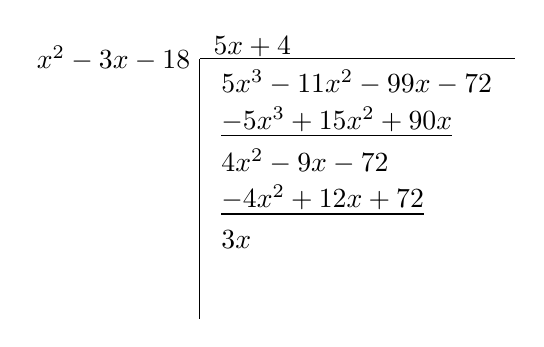
\begin{tikzpicture}[baseline=(current bounding box.north)]
  % Division Bar
  \draw (0,0) -- (0,-3.3); % vertical bar
  \draw (0,0) -- (4,0); % horizontal bar
  % Divisor
  \node[anchor=east] at (0,0) {$x^2 - 3x - 18$};
  % Dividend (aligned below the bar)
  \node[anchor=west] at (0.05,0.15) {$5x+4$};
  \node[anchor=west] at (0.15,-0.3) {$5x^3 - 11x^2 - 99x - 72$};
  \node[anchor=west] at (0.15,-0.8) {$\underline{-5x^3 + 15x^2 + 90x}$};
  \node[anchor=west] at (0.15,-1.3) {$4x^2 - 9x - 72$};
  \node[anchor=west] at (0.15,-1.8) {$\underline{-4x^2 + 12x + 72}$};
  \node[anchor=west] at (0.15,-2.3) {$3x$};
\end{tikzpicture}
\]

Test 5

\[\begin{array}{r@{} r@{} r@{} r }
  5x^3 &{}-11x^2 &{}\Ph-99x&{}-72   \\
 -5x^3 &{}+15x^2 &{}\Ph+90x&\\
\cmidrule{1-3}
       &{}\Ph4x^2&{}+\Ph9x &{}-72\\
       &{}-  4x^2&{}+ 12x  &{}+72 \\
\cmidrule{2-4}
       &         &{}\Ph3x  &{} \\
\end{array}\]

test 6

\[\begin{array}{rr}
    5x & +4\\
    \begin{array}{r@{} r@{} r@{}|r@{} r@{} r@{} r}
        \cmidrule{4-7}
    x^2 & -3x & -18 & 5x^3 & -11x^2 & -99x & -72 \\
\begin{array}{r@{} r@{} r@{} r }
  5x^3 &{}-11x^2 &{}\Ph-99x&{}-72   \\
 -5x^3 &{}+15x^2 &{}\Ph+90x&\\
\cmidrule{1-3}
       &{}\Ph4x^2&{}+\Ph9x &{}-72\\
       &{}-  4x^2&{}+ 12x  &{}+72 \\
\cmidrule{2-4}
       &         &{}\Ph3x  &{} \\
\end{array}
\end{array}
\end{array}\]

test 7

\[
\setlength{\arraycolsep}{3pt}
\renewcommand{\arraystretch}{1.2}
\begin{array}{rl|l}
  & 5x+4 & \\[-1.5ex]
  x^2-3x-18 & \multicolumn{2}{l}{\big)} 5x^3 - 11x^2 - 99x - 72 \\ \cline{2-3}
  & -5x^3 + 15x^2 + 90x \\[-1ex]
  & 4x^2 - 9x - 72 \\
  & -4x^2 + 12x + 72 \\[-1ex]
  & 3x
\end{array}
\]

test 8

\[
\setlength{\arraycolsep}{3pt}
\renewcommand{\arraystretch}{1.2}
\begin{array}{r|l}
  5x + 4 & \\[-1.5ex]
  x^2-3x-18\,\,\,\Big| & 5x^3 - 11x^2 - 99x - 72 \\ \cline{2-2}
  & -5x^3 + 15x^2 + 90x \\[-1ex]
  & \phantom{-}4x^2 - 9x - 72 \\
  & -4x^2 + 12x + 72 \\[-1ex]
  & \phantom{-}3x
\end{array}
\]

Test 9

\[
\setlength{\arraycolsep}{2pt}
\renewcommand{\arraystretch}{1.3}
\begin{array}{r@{}c@{}l}
    & 5x+4 & \\[0.5ex]             % Quotient (answer) above dividend
    x^2 - 3x - 18\,\,\bigg| & \hspace{-0.6em} & 5x^3 - 11x^2 - 99x - 72 \\[-0.6ex] % divisor and dividend, with bar
    \cline{2-3}
    && -5x^3 + 15x^2 + 90x \\
    && 4x^2 - 9x - 72 \\
    && -4x^2 + 12x + 72 \\
    && 3x \\
\end{array}
\]

Test 10

\[
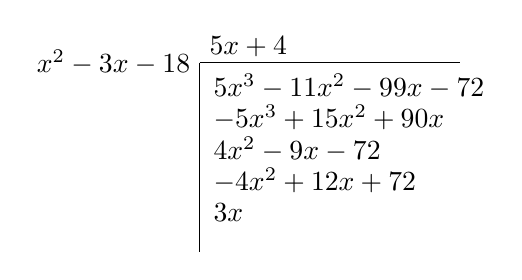
\begin{tikzpicture}[baseline={(current bounding box.north)}]
    % vertical bar
    \draw (0,0) -- (0,-2.4);
    % horizontal bar (for the answer)
    \draw (0,0) -- (3.3,0);
    % nodes
    \node[anchor=west] at (0, 0.2) {$5x+4$};
    \node[anchor=east] at (0, 0) {$x^2 - 3x - 18$};
    \node[anchor=west] at (0.05, -0.3) {$5x^3 - 11x^2 - 99x - 72$};
    \node[anchor=west] at (0.05, -0.7) {$-5x^3 + 15x^2 + 90x$};
    \node[anchor=west] at (0.05, -1.1) {$4x^2 - 9x - 72$};
    \node[anchor=west] at (0.05, -1.5) {$-4x^2 + 12x + 72$};
    \node[anchor=west] at (0.05, -1.9) {$3x$};
\end{tikzpicture}
\]

Test 11

\[
\setlength{\arraycolsep}{2pt}
\renewcommand{\arraystretch}{1.3}
\begin{array}{r@{}c@{}l}
   & 5x+4 & \\[0.5ex]
   x^2 - 3x - 18\,\,\bigg| & \hspace{-0.6em} & 5x^3 - 11x^2 - 99x - 72 \\[-0.6ex]
   \cline{2-3}
   && -5x^3 + 15x^2 + 90x\phantom{\, - 72} \\
   && \phantom{-}4x^2 - 9x - 72\phantom{00000} \\
   && -4x^2 + 12x + 72\phantom{00} \\
   && \phantom{-4x^2 + 12x + 72}3x \\
\end{array}
\]

Test 12

\[\myPolyDiv2{5x^{3}-11x^{2}-99x-72}{x^{2}-3x-18}\]

Test 13

\[
\begin{array}{rrrrrrr}
  \Ph  & \Ph & \Ph & \Ph & \Ph & 5x & +4\\
  \begin{array}{rrr|rrrr}
\cmidrule{4-7}
x^2 & -3x & -18 & 5x^3 & -11x^2 & -99x & -72 \\
\begin{array}{rrrrrrr}
  \Ph  &  \Ph   &  \Ph   & -5x^3& +15x^2 & +90x & \\
\cmidrule{4-6}  
  \Ph  &   \Ph  &  \Ph   &  \Ph    &  4x^2 & -9x  & -72 \\
   \Ph &  \Ph   & \Ph    &  \Ph    & -4x^2 & +12x & +72 \\
\cmidrule{5-7}
  \Ph  &  \Ph   &  \Ph   &  \Ph    &  \Ph     & 3x & 0 \\
\end{array}
\end{array}
\end{array}\]

 Test 14

 \[
\begin{array}{r@{}r@{}r@{}r@{}r@{}r@{}r@{}}
  \Ph  & \Ph & \Ph & \Ph & \Ph & 5x & +4\\
\begin{array}{r@{}r@{}r@{}|r@{}r@{}r@{}r@{}}
\cmidrule{4-7}
x^2 & -3x & -18 & 5x^3 & -11x^2 & -99x & -72 \\
\begin{array}{r@{}r@{}r@{}r@{}r@{}r@{}r@{}}
  \Ph  &  \Ph   &  \Ph   & -5x^3& +15x^2 & +90x & \\
\cmidrule{4-6}  
  \Ph  &   \Ph  &  \Ph   &  \Ph    &  4x^2 & -9x  & -72 \\
   \Ph &  \Ph   & \Ph    &  \Ph    & -4x^2 & +12x & +72 \\
\cmidrule{5-7}
  \Ph  &  \Ph   &  \Ph   &  \Ph    &  \Ph     & 3x &  \\
\end{array}
\end{array}
\end{array}\]

test 15

Hi Joanne, 

I am getting in touch about the typesettig of my polynomial long division. I am using 
\LaTeX\ and my long division looks very much like the polylongdiv command from the 
polynum package. However, this is simply because that is how I want it to look. So I am 
sending you the code inadvance so you can see I am doing it by hand and not relying on
the package. Is this Okay?, Obviously not if the answer is correct, but jsut if I can
use the same layout as the polylongdiv command.

\[\begin{array}{r@{} r@{} r@{} r@{} r@{} r@{} r@{}}
    {}  & {} & {} & {} & {} & 5x & +4\\
\cmidrule{4-7}
   x^2 & -3x & -18\big) & 5x^3 & -11x^2 & -99x & -72 \\
    {}  &  {}   &  {}   & -5x^3& +15x^2 & +90x & \\
\cmidrule{4-6}  
  {}  &   {}  &  {}   &  {}    &  4x^2 & -9x  & -72 \\
  {} &  {}   & {}    &  {}    & -4x^2 & +12x & +72 \\
\cmidrule{5-7}
  {}  &  {}   &  {}   &  {}    &  {}     & 3x &  \\
\end{array}\]

Test 16

\[
\begin{array}{r@{\hspace{0.2em}}l}
\multicolumn{2}{l}{\hspace{2em}5x + 4} \\
\cline{2-2}
x^2 - 3x - 18\,)\! & 5x^3 - 11x^2 - 99x - 72 \\
 & -5x^3 + 15x^2 + 90x \\
\cline{2-2}
 & \phantom{-}4x^2 - 9x - 72 \\
 & -4x^2 + 12x + 72 \\
\cline{2-2}
 & \phantom{-}3x
\end{array}
\]

ideal

\polylongdiv{5x^{3}-11x^{2}-99x-72}{x^{2}-3x-18}


Next test can I generalise this?

Ideal

\polylongdiv{27x^3+9x^2-3x-10}{3x-2}



Test 1

\[\begin{array}{r@{} r@{} r@{} r@{} r@{} r@{}}
     {} & {} & {} & 9x^2 & +9x & +4\\
\cmidrule{3-6}
    3x & -2\big) & 27x^3 & +9x^2 & -3x & -10 \\
    {}  &  {}   &  -27x^3 & +18x^2 & {} & {}  \\
\cmidrule{3-4}  
  {}  &   {}  &  {}   &  27x^2  &  -3x & {} \\
  {} &  {}   & {}    &  -27x^2    & +18x & {} \\
\cmidrule{4-5}
  {}  &  {}   &  {}   &  {}    & 15x & -10    \\
    {}  &  {}   &  {}   &  {}    & -15x & +10 \\
\cmidrule{5-6}
    {}  &  {}   &  {}   &  {}    & {}     & 0 \\
\end{array}\]


\end{document}